%%
%% Do Small Proxy Models Know When GPT-3 Hallucinates?
%% Implementation study (Paper 2, AI Tools for Research). acmart, acmsmall, like Paper 1.
%%
\documentclass[acmsmall,screen,review,nonacm]{acmart}

\AtBeginDocument{%
  \providecommand\BibTeX{{%
    Bib\TeX}}}

\setcopyright{none}
\settopmatter{printacmref=false}

\usepackage{tabularx}
\usepackage{multirow}
\usepackage{tikz}
\usetikzlibrary{shapes.geometric, arrows.meta, positioning}
\newcommand{\nf}{\textsc{NonFact}}

\begin{document}

\title[Proxy Token Uncertainty for Hallucination Detection]{Do Small Proxy Models Know When GPT-3 Hallucinates? A Controlled Study of Token-Level Uncertainty, Semantic-Anchor Weighting and Two-Stage Screening}

\author{Aman Bhagat}
\email{MCL2026013@gmail.com}
\affiliation{%
  \institution{Indian Institute of Information Technology Allahabad (IIITA)}
  \city{Prayagraj}
  \state{Uttar Pradesh}
  \country{India}
}
\renewcommand{\shortauthors}{Aman Bhagat}

\begin{abstract}
Bluntly, my earlier literature review argued token log-probabilities and entropies are a cheap but partial signal of hallucination, and suggested two untested ideas: weighting only the \emph{semantic-anchor} tokens of a claim (names, numbers, dates), and a \emph{two-stage} design in which a token score is deciding which sentences receive an expensive semantic check, in many respects. This paper tests both in the setting that matters for closed APIs, where the generator's own probabilities are unavailable and must be estimated by a small open \emph{proxy} model, on the whole. On the SelfCheckGPT WikiBio benchmark (238 GPT-3 passages, 1{,}908 annotated sentences) I first reproduce the random baseline exactly (72.96 AUC-PR) and SelfCheckGPT-NLI to, within 0.01 points (92.50 vs.\ 92.50 reported). I then score the same text with six proxies of 0.5B--3B parameters from three families; in fact, every pre-specified proxy score is at or below the random baseline (66.3--74.2 AUC-PR); the log-probability scores are \emph{inverted} (AUROC 40--43): proxies find hallucinated sentences \emph{more} predictable than correct ones. Anchor weighting is raising Avg($-\log p$) by 2.3--3.3 AUC-PR points in all six proxies (95\% bootstrap CIs exclude zero) and beats SAR relevance weighting, but an AUROC analysis suggests the gain comes from cancelling the inverted signal, not from detecting hallucinations; a pre-specified two-stage cascade is therefore no better than routing sentences at random. An exploratory diagnosis locates the inversion between passages: fully fabricated biographies are generic and easy to predict. Within a passage proxy uncertainty carries almost no information (AUROC 48--53); these outcomes are arguing against employing small proxy models as hallucination screens and in favour of sampling-based checks or the generator's own probabilities.
\end{abstract}

\begin{CCSXML}
<ccs2012>
 <concept>
  <concept_id>10010147.10010178.10010179</concept_id>
  <concept_desc>Computing methodologies~Natural language processing</concept_desc>
  <concept_significance>500</concept_significance>
 </concept>
</ccs2012>
\end{CCSXML}
\ccsdesc[500]{Computing methodologies~Natural language processing}

\keywords{hallucination detection, token-level uncertainty, proxy language models, SelfCheckGPT, semantic-anchor weighting, reproducibility, negative results}

\maketitle

%% ------------------------------------------------------------------
\section{Introduction}

On the page, a fluent wrong sentence and a fluent right sentence look the same, to a significant degree. In my literature review~\cite{bhagat2026review} I inspected whether the model's own next-token distribution can tell them apart, and concluded token log-probability and entropy are \textquotedblleft a real but partial predictor\textquotedblright - on GPT-3 biographies the single most surprising token of a sentence already is lifting AUC-PR from 72.96 (random) to 87.51, but sampling-based checks reach 93.42~\cite{manakul2023selfcheckgpt}, broadly speaking. The review closed with a research agenda. Two of its proposals are tested here: \emph{semantic-anchor weighting} (Sec.~8.2 of the review), a cheaper alternative to SAR relevance weighting~\cite{duan2024shifting} that's keeping only the tokens of entities, numbers and dates; and a \emph{two-stage early-warning architecture} (Sec.~8.3), where a token score flags spans and only flagged spans are sent to an expensive semantic check.

As, well, both proposals quietly suppose that token probabilities are \emph{available}, and for most people commercial APIs they aren't, or only as shortened top-$k$ lists, in actual application; the concrete alternative, also reported in the SelfCheckGPT paper, is to re-score the created text with an open \emph{proxy} model, in real-world scenarios. In that paper a LLaMA-30B proxy reached 75.43--80.92 AUC-PR, smaller proxies were near or below random, and max($-\log p$) matched up \emph{negatively} with human passage scores~\cite{manakul2023selfcheckgpt}, and the review listed model dependence and cross-model calibration as open gaps (Secs.~6.4, 7); this study is asking what happens to the review's two proposals when they have to run on a small stand-in that's fitting on a free GPU.

\paragraph{Research questions.}
\begin{description}
  \item[RQ1] When the generator's probabilities are unavailable, how well do token-level uncertainty scores from open proxy LMs of 0.5B--3B parameters detect non-factual sentences, and how does this rest on proxy size, family and the aggregation rule?
  \item[RQ2] Does semantic-anchor weighting, or SAR relevance weighting, improve on the plain token average?
  \item[RQ3] And more, can, in practice, maybe a token-score screen route only a fraction of sentences to SelfCheckGPT-NLI while keeping more of its quality than routing at random?
\end{description}

\paragraph{Contributions.} (i) A validated, reproducible baseline: the random baseline is reproduced exactly and SelfCheckGPT-NLI to within 0.01 AUC-PR, with an equivalence check against the official scoring logic (Sec.~\ref{sec:validation}). (ii) A controlled comparison of eight scoring rules across six proxy LMs under one frozen protocol, with passage-level bootstrap confidence intervals (Sec.~\ref{sec:rq1}). (iii) The first test of the review's anchor-weighting proposal, with an ablation over the non-anchor weight (Sec.~\ref{sec:rq2}). (iv) A cost--quality evaluation of the two-stage design against a random-routing control (Sec.~\ref{sec:rq3}). (v) An exploratory error analysis that explains the negative result (Sec.~\ref{sec:diag}). The intended contribution is evidence, not a new detector; the main findings are negative and are reported as such.

%% ------------------------------------------------------------------
\section{Related Work}
\label{sec:related}

\paragraph{Token-level uncertainty.} Malinin and Gales~\cite{malinin2021uncertainty} set out token- and sequence-level uncertainty measures for autoregressive models; LM-Polygraph~\cite{lmpolygraph} benchmarks them, with likelihood and entropy as standard white-box baselines. The survey by Shorinwa et al.~\cite{uqsurvey2025} warns that token confidence can be miscalibrated. My review~\cite{bhagat2026review} summarises this line of work and its limits.

\paragraph{SelfCheckGPT} Manakul et al.~\cite{manakul2023selfcheckgpt} released the WikiBio hallucination data used here (GPT-3 passages about WikiBio~\cite{lebret2016wikibio} subjects, sentence-level human labels, 20 stochastic samples per passage). They compared grey-box scores from GPT-3's own probabilities, black-box scores from proxy LMs (LLaMA, OPT, GPT-J, NeoX), and sampling-based consistency checks. Their NLI variant scores each sentence by the mean probability that a DeBERTa-v3-large MNLI model~\cite{he2023debertav3} labels it as contradicted by a sample.

\paragraph{Relevance weighting and semantic uncertainty.} SAR~\cite{duan2024shifting} re-weights token uncertainty by how much the meaning of an answer changes when the token is removed, measured with a cross-encoder~\cite{reimers2019sbert}. Semantic entropy~\cite{kuhn2023semantic,farquhar2024semantic} measures uncertainty over clusters of equivalent answers. Both point away from the plain token average. Neither has been tested with a proxy model on long-form text, and the anchor-only variant proposed in the review has not been tested at all.

%% ------------------------------------------------------------------
\section{Method}
\label{sec:method}

\subsection{Task, data and protocol}
What's more, each of the 1{,}908 GPT-3 sentences is labelled \emph{accurate} (516), \emph{minor-inaccurate} (631) or \emph{major-inaccurate} (761), in many respects; indeed, passage-level agreement is the Pearson/Spearman correlation between the mean human score (accurate 0, minor 0.5, major 1) and the mean sentence score, in actual application. \nf{}* detects major-inaccurate sentences after removing the passages in which \emph{every} sentence is major-inaccurate (1{,}632 sentences remain); and thus, Following SelfCheckGPT, the primary task \nf{} treats both inaccurate classes as positive (72.96\% positives), so on top of that, \emph{Factual} detects accurate sentences, employing the negated score. The dataset is used purely as a test set, including nothing is trained, and every design choice and the primary metric (\nf{} AUC-PR, computed with \texttt{precision\_recall\_curve} and trapezoidal \texttt{auc} exactly as in the SelfCheckGPT code) were fixed in \texttt{configs/experiment.yaml} before any score was computed.

\subsection{Proxy token scores}
A proxy LM is reading a fixed prefix (\textquotedblleft\textit{The following is a Wikipedia biography.}\textquotedblright) followed by the full GPT-3 passage, in one deterministic fp16 forward pass, broadly speaking; and thus, a 7B model doesn't fit on the 16\,GB T4 GPU in fp16, which is setting the upper size limit, in real-world scenarios. Each token is typically named to the sentence and whitespace word that's comprising its first non-space character (character offsets from the fast tokenizer); 15--19 inter-sentence tokens per model can't be handed out and are generally dropped; each token $y_t$ of the passage it's giving $-\log p(y_t\mid\cdot)$ and the full-vocabulary entropy $H_t$ (Eq.~1 of the review). Six proxies are covering three families and a size range - Qwen2.5-0.5B, -1.5B, -3B and -1.5B-Instruct~\cite{qwen2025qwen25}, OPT-1.3B~\cite{zhang2022opt} and Pythia-1.4B~\cite{biderman2023pythia}; in fact, sentence scores are the mean and maximum of $-\log p$ and of $H$ (Avg/Max), as in SelfCheckGPT.

\subsection{Relevance and anchor weighting (RQ2)}
\emph{SAR comparator.} Following Duan et al.~\cite{duan2024shifting}, the relevance of word $w_i$ is $R_i = 1 - \mathrm{sim}(s, s\setminus w_i)$, where \nolinkurl{cross-encoder/stsb-roberta-large} supplies the similarity, in actual application, and removal is usually done at the word level rather than the token level, so that one relevance vector serves all six tokenizers (33{,}372 sentence pairs), in actual application. What's more, every token inherits the relevance of its word; in turn, the SAR score is the relevance-weighted mean of $-\log p$ or $H$.

\emph{Semantic-anchor weighting (the modification under test).} spaCy~\cite{honnibal2020spacy} (\texttt{en\_core\_web\_sm}) is marking a word as an anchor if it overlaps a token tagged PROPN or NUM, or a named item of any of 18 types (PERSON, ORG, GPE, DATE, CARDINAL, \ldots), broadly speaking; indeed, anchors are making up 35.9\% of words, and 92 sentences have none. The anchor score is normally $\sum_t w_t u_t / \sum_t w_t$ with $w_t = 1$ for anchor tokens and $w_t=\alpha$ otherwise, where $u_t \in \{-\log p, H\}$, broadly speaking; and thus, the primary setting $\alpha = 0$ (anchors only; plain mean if a sentence has no anchors) was fixed in advance; $\alpha \in \{0.1, 0.25, 0.5, 1\}$ is an ablation. What's more, $\alpha=1$ recovers the plain average. Unlike SAR, this needs no second neural model beyond a small tagger.

\subsection{Comparator and two-stage cascade (RQ3)}
SelfCheckGPT-NLI is currently re-implemented in batched fp16 form with the released \nolinkurl{potsawee/deberta-v3-large-mnli} model. What's more, flagged sentences are often ranked above unflagged ones; unflagged sentences are keeping their stage-1 rank, on the whole. In the cascade, the top-$q$ fraction of sentences by a stage-1 token score is mainly re-scored by NLI, to a significant degree. All 1{,}908$\times$20 = 38{,}160 (sentence, sample) contradiction probabilities are stored, so the score for $N<20$ samples can be read off without re-running the model. The stage-1 score was fixed in advance as Avg($H$) of the largest proxy (Qwen2.5-3B), because Avg($H$) was the strongest proxy score family in SelfCheckGPT's Table~2. A random $q$ fraction is instead routed by the control, with 10 seeds.

\subsection{Statistics and implementation}
Uncertainty is estimated with a 1{,}000-resample bootstrap over \emph{passages} (seed 0), because sentences, within a passage aren't autonomous, on the whole; and thus, all runs employed Google Colab with one Tesla T4 (16\,GB), Python 3.13, PyTorch 2.14.1, Transformers 5.22.1 and sentence-transformers 5.7.0, in actual application. Differences between scoring rules are paired, computed on the same resamples; and thus, code, setup, logs, per-sentence scores and the commands to regenerate every table and figure are in the accompanying repository.

%% ------------------------------------------------------------------
\section{Baseline Validation}
\label{sec:validation}

\begin{table}[t]
  \caption{Baseline validation against the values reported by Manakul et al.~\cite{manakul2023selfcheckgpt} (Table~2). AUC-PR and correlations $\times 100$.}
  \label{tab:validation}
  \footnotesize
  \begin{tabular}{lrrrrr}
    \toprule
    & \nf{} & \nf{}* & Factual & Pearson & Spearman \\
    \midrule
    Random baseline, reported & 72.96 & 29.72 & 27.04 & -- & -- \\
    Random baseline, this study & 72.96 & 29.72 & 27.04 & -- & -- \\
    SelfCheckGPT-NLI ($N{=}20$), reported & 92.50 & 45.17 & 66.08 & 74.14 & 73.78 \\
    SelfCheckGPT-NLI ($N{=}20$), this study & 92.50 & 45.16 & 66.08 & 74.13 & 73.77 \\
    \bottomrule
  \end{tabular}
\end{table}

Table~\ref{tab:validation} shows the finding. The published positive rates are exactly reproduced by the label counts (761/631/516), which also is corroborating the \nf{}* definition, such as removing fully hallucinated passages gives the published 29.72\% major-inaccurate rate, in actual application; indeed, SelfCheckGPT-NLI is, in effect, matching the published numbers to within 0.01 points on every metric. The formal \texttt{selfcheckgpt} 0.1.7 package couldn't be imported, under Transformers 5 (it calls the removed \texttt{batch\_encode\_plus}), on the whole; indeed, its scoring logic (one unpadded pair per forward pass in fp32) was therefore re-implemented line by line and compared with the batched fp16 version on the first five passages (45 sentences $\times$ 20 samples). The maximum absolute difference in sentence scores was $4.4\times10^{-4}$ (Pearson $r>0.9999$), and the baseline is therefore considered checked. What's more, its AUROC (83.69) and per-$N$ results below are new measurements on a checked implementation.

%% ------------------------------------------------------------------
\section{Results}
\label{sec:results}

\begin{table*}[t]
  \caption{Sentence-level \nf{} AUC-PR for eight token scores and six proxy LMs (random: 72.96; SelfCheckGPT-NLI: 92.50). Values above the random baseline are in bold. The last three columns give AUROC, \nf{}* AUC-PR and passage-level Pearson $r$ ($\times100$) for Avg($-\log p$). For comparison, SelfCheckGPT reports Avg($-\log p$) of 83.21 with GPT-3's own probabilities and 71.69--75.43 with LLaMA-7B/30B proxies.}
  \label{tab:main}
  \footnotesize
  \setlength{\tabcolsep}{3.6pt}
  \resizebox{\textwidth}{!}{%
  \begin{tabular}{l rrrr rr rr | rrr}
    \toprule
    & \multicolumn{4}{c}{plain aggregation} & \multicolumn{2}{c}{SAR-weighted} & \multicolumn{2}{c|}{anchor-weighted ($\alpha{=}0$)} & \multicolumn{3}{c}{Avg($-\log p$)} \\
    Proxy LM & Avg($-\log p$) & Max($-\log p$) & Avg($H$) & Max($H$) & $-\log p$ & $H$ & $-\log p$ & $H$ & AUROC & \nf{}* & Pearson \\
    \midrule
    Qwen2.5-0.5B & 66.34 & 68.71 & 69.46 & 72.21 & 66.94 & 68.90 & 68.95 & 70.30 & 39.96 & 23.18 & $-$46.7 \\
    Qwen2.5-1.5B & 67.30 & 68.95 & 70.54 & 72.83 & 68.47 & 70.29 & 70.33 & 71.79 & 41.72 & 22.93 & $-$43.2 \\
    Qwen2.5-3B   & 68.37 & 70.16 & 70.65 & \textbf{74.19} & 69.19 & 70.48 & 70.70 & 72.50 & 42.80 & 22.77 & $-$39.2 \\
    Qwen2.5-1.5B-Inst & 67.54 & 69.03 & 70.81 & 72.89 & 68.65 & 70.54 & 70.54 & 72.10 & 42.34 & 23.01 & $-$42.4 \\
    OPT-1.3B     & 66.89 & 68.90 & 72.06 & \textbf{73.70} & 68.27 & 72.01 & 70.21 & 72.88 & 41.25 & 22.59 & $-$44.9 \\
    Pythia-1.4B  & 67.04 & 68.09 & 72.56 & \textbf{73.52} & 68.61 & 72.76 & 70.38 & \textbf{73.23} & 40.78 & 22.32 & $-$49.0 \\
    \bottomrule
  \end{tabular}}
\end{table*}

\begin{figure}[t]
  \centering
  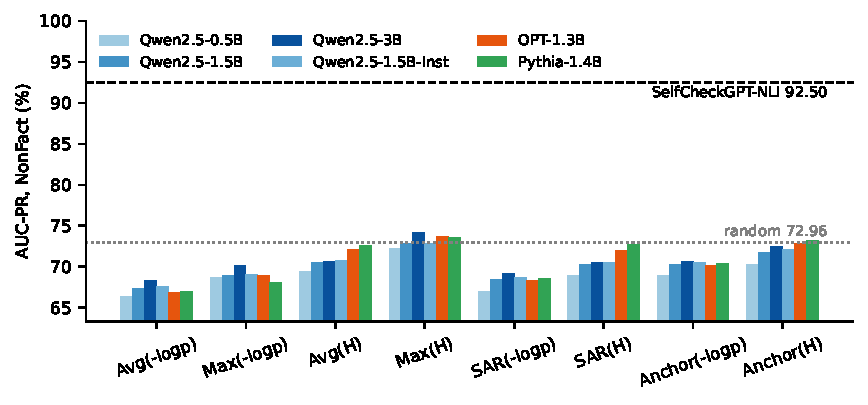
\includegraphics[width=\linewidth]{figures/fig_main_aucpr.pdf}
  \caption{\nf{} AUC-PR of every proxy score (bars) against the random baseline (dotted) and the validated SelfCheckGPT-NLI baseline (dashed).}
  \Description{Grouped bar chart. For eight scoring rules and six proxy models, all bars lie between about 66 and 74 AUC-PR, around or below a dotted random line at 72.96 and far below a dashed line at 92.50 for SelfCheckGPT-NLI.}
  \label{fig:main}
\end{figure}

\subsection{RQ1: proxy token scores do not detect hallucinations}
\label{sec:rq1}
Table~\ref{tab:main} and Figure~\ref{fig:main} answer RQ1. Of the 48 combinations of proxy and pre-specified score, only four exceed the random baseline, in actual application. All four are Max($H$) or Anchor($H$) and exceed it by at most 1.23 points: Qwen2.5-3B Max($H$) 74.19, OPT-1.3B 73.70, Pythia-1.4B 73.52 and Pythia-1.4B Anchor($H$) 73.23. For the strongest anchor score the bootstrap interval (Qwen2.5-3B Anchor($H$): 68.3--76.7) comprises the random rate; the log-probability scores are clearly \emph{below} random. Their AUROC is 40--43, below 50 for all six proxies. Still. Their passage-level link with human scores is negative ($-$39 to $-$49); this reproduces, for a new set of proxies, the direction SelfCheckGPT reported for LLaMA Max($-\log p$) (Pearson $-$22.8 to $-$42.6). Scaling the proxy helps only slightly: within the Qwen2.5 family, Avg($-\log p$) rises from 66.34 (0.5B) to 68.37 (3B). Instruction tuning changes little (67.30 vs.\ 67.54 at 1.5B), and entropy scores are consistently less inverted than log-probability scores. Table~\ref{tab:dist} shows the system directly - for every proxy, major-inaccurate sentences have \emph{lower} mean $-\log p$ and $H$ than accurate ones.

\begin{table}[t]
  \caption{Mean sentence score by human label (Avg($-\log p$) / Avg($H$), nats). Hallucinated sentences are the \emph{more} predictable ones. The scale also differs by 0.5 nats across proxies.}
  \label{tab:dist}
  \footnotesize
  \begin{tabular}{lccc}
    \toprule
    Proxy & accurate & minor-inacc. & major-inacc. \\
    \midrule
    Qwen2.5-0.5B & 1.594 / 2.100 & 1.491 / 2.031 & 1.287 / 1.940 \\
    Qwen2.5-3B & 1.183 / 1.589 & 1.165 / 1.592 & 0.946 / 1.461 \\
    OPT-1.3B & 1.535 / 2.145 & 1.470 / 2.159 & 1.247 / 2.066 \\
    Pythia-1.4B & 1.478 / 2.076 & 1.425 / 2.104 & 1.197 / 2.005 \\
    \bottomrule
  \end{tabular}
\end{table}

\subsection{RQ2: anchor weighting helps, but for the wrong reason}
\label{sec:rq2}

\begin{table}[t]
  \caption{Paired passage-bootstrap differences in \nf{} AUC-PR (point estimate [95\% CI], 1{,}000 resamples). Intervals that exclude zero are in bold.}
  \label{tab:paired}
  \footnotesize
  \setlength{\tabcolsep}{3pt}
  \begin{tabular}{lccc}
    \toprule
    Proxy & Anchor$-$Avg ($-\log p$) & SAR$-$Avg ($-\log p$) & Anchor$-$SAR ($H$) \\
    \midrule
    Qwen2.5-0.5B & \textbf{+2.61} [1.28, 4.22] & +0.60 [$-$0.36, 1.49] & \textbf{+1.40} [0.08, 2.63] \\
    Qwen2.5-1.5B & \textbf{+3.03} [1.51, 4.67] & \textbf{+1.17} [0.22, 2.03] & \textbf{+1.50} [0.27, 2.71] \\
    Qwen2.5-3B & \textbf{+2.33} [0.88, 3.88] & +0.83 [$-$0.05, 1.70] & \textbf{+2.02} [0.75, 3.18] \\
    Qwen2.5-1.5B-Inst & \textbf{+3.00} [1.55, 4.62] & \textbf{+1.11} [0.20, 1.98] & \textbf{+1.56} [0.28, 2.78] \\
    OPT-1.3B & \textbf{+3.32} [1.65, 5.03] & \textbf{+1.38} [0.43, 2.33] & +0.88 [$-$0.79, 2.31] \\
    Pythia-1.4B & \textbf{+3.33} [1.68, 4.99] & \textbf{+1.57} [0.64, 2.44] & +0.47 [$-$1.12, 1.88] \\
    \bottomrule
  \end{tabular}
\end{table}

\begin{figure}[t]
  \centering
  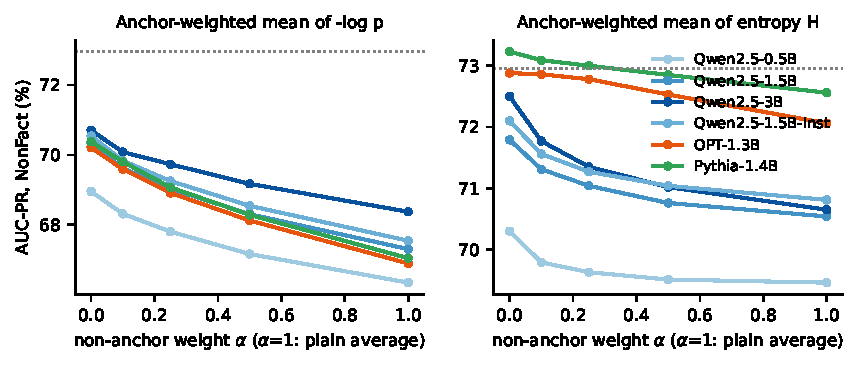
\includegraphics[width=\linewidth]{figures/fig_alpha_sensitivity.pdf}
  \caption{Ablation of the non-anchor weight $\alpha$. $\alpha{=}1$ is the plain average; $\alpha{=}0$ uses anchor tokens only.}
  \Description{Two line plots. For every proxy, AUC-PR decreases monotonically as alpha increases from 0 to 1, for both log-probability (left) and entropy (right). All curves stay at or below the random line at 72.96.}
  \label{fig:alpha}
\end{figure}

The largest and most uniform change in the study is being given by anchor weighting, broadly speaking. Restricting Avg($-\log p$) to anchor tokens raises \nf{} AUC-PR by 2.3--3.3 points in all six proxies, and every 95\% CI excludes zero (Table~\ref{tab:paired}); it also outperforms the SAR comparator in four of six proxies for entropy and in all six for $-\log p$ (anchor$-$SAR for $-\log p$: +1.5 to +2.0, all CIs are excluding zero), on the whole. SAR's own gain over the plain average is generally smaller (+0.6 to +1.6 for $-\log p$) and vanishes for entropy, where all six differences straddle zero ($-$0.56 to +0.20); the ablation in Figure~\ref{fig:alpha} is monotone for every proxy - the less weight on non-anchor tokens, the higher the AUC-PR, with $\alpha{=}0$ best.

Read naively, this would validate the review's hypothesis. The AUROC and correlation columns don't: Anchor($H$) is moving AUROC from 44.7--49.0 (Avg($H$)) to 46.5--50.7, and the passage correlation from $-$11 to $-$21 to between $-$10 and 0 (e.g.\ Qwen2.5-3B: $-$19.5 to $+$0.2), on the whole. Anchor weighting doesn't add positive indication of falsehood; so, it removes most of an inverted signal and pushes the scores towards the chance, to a significant degree. As, AUC-PR on a 73\%-positive task punishes inverted rankings more than random ones, moving towards the chance looks like an enhancement; and thus, the answer to RQ2 is therefore that anchor weighting is consistently (specifically in this setting) \emph{less wrong} than the plain average and than SAR. None of the three is, for all practical purposes, a usable detector with proxies of this size.

\begin{figure}[t]
  \centering
  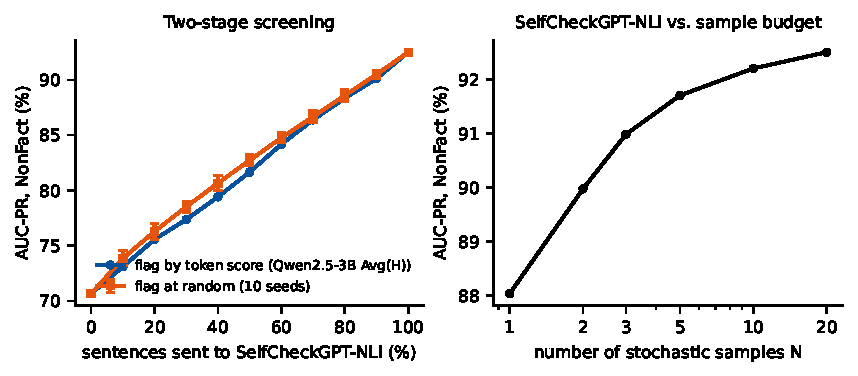
\includegraphics[width=\linewidth]{figures/fig_cascade_nli.pdf}
  \caption{Left: two-stage screening. Sentences flagged by the pre-specified token score (blue) or at random (orange, mean $\pm$ s.d.\ over 10 seeds) are re-scored by SelfCheckGPT-NLI. Right: SelfCheckGPT-NLI as a function of the number of samples.}
  \Description{Left: two almost linear curves rising from 70.6 to 92.5 AUC-PR as the fraction of sentences sent to NLI goes from 0 to 100 percent. The token-score curve lies slightly below the random-routing curve at every fraction. Right: NLI AUC-PR rises from 88.0 with one sample to 92.5 with twenty, flattening after five.}
  \label{fig:cascade}
\end{figure}

\subsection{RQ3: a two-stage screen cannot be built on an inverted score}
\label{sec:rq3}
Seeing as the stage-1 score is inverted, the cascade (Fig.~\ref{fig:cascade}, left) does no better than random routing, to a significant degree. At every budget the token-score selector is 0.25--1.24 points \emph{below} the random-routing mean, such as to take one instance, 81.65 against 82.72 ($\pm$0.51) when half the sentences are currently re-scored, broadly speaking. At that budget it represents 48.6\% of the non-factual sentences, against 50.3\% for random selection. As an exploratory check, using the best observed proxy score (Qwen2.5-3B Max($H$)) as the selector instead gives differences of $-$0.54 to $+$0.27 points against random routing, so the conclusion does not depend on the pre-specified selector. Quality rises almost linearly with the fraction re-scored. In a place like this the cost saving of a two-stage design is simply the fraction not re-scored, with a proportional loss of quality.

A cheaper way to decrease cost is shown by the right-hand panel: SelfCheckGPT-NLI with $N{=}5$ samples keeps 91.70 of its 92.50 AUC-PR (and 3 samples keep 90.98) at a quarter of the sampling and NLI cost. Measured on the T4, NLI took 680\,s for all 38{,}160 pairs, or 0.36\,s per sentence at $N{=}20$, while a full proxy pass took 9--27\,s for all 1{,}908 sentences, or 5--14\,ms per sentence. The token score is about 25--70 times cheaper, but cost only matters once a score carries signal.

%% ------------------------------------------------------------------
\section{Error Analysis and Diagnosis}
\label{sec:diag}

\begin{figure}[t]
  \centering
  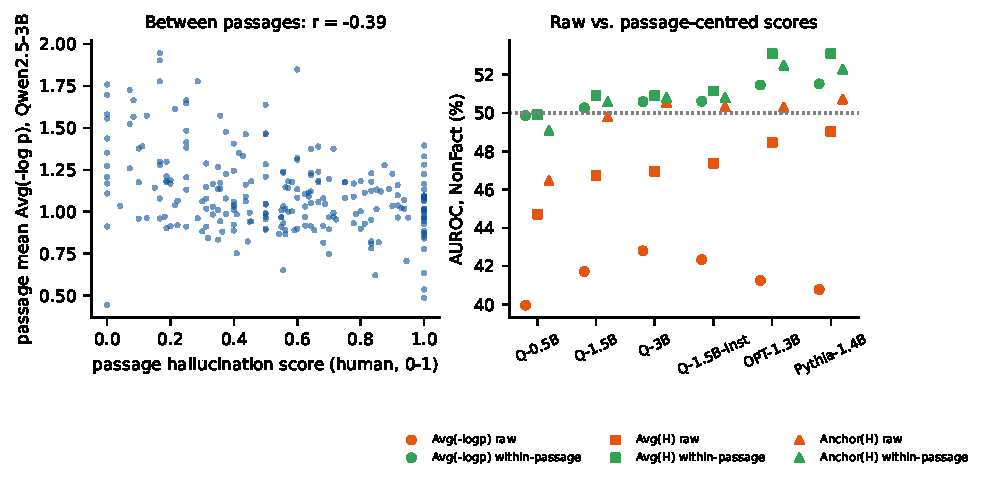
\includegraphics[width=\linewidth]{figures/fig_passage_confound.pdf}
  \caption{Exploratory diagnosis. Left: across passages, the more a passage is hallucinated, the lower its mean surprise under Qwen2.5-3B. Right: AUROC of raw scores (orange) and of scores centred on their passage mean (green). After centring, every proxy is at chance.}
  \Description{Left: scatter of 238 passages; mean negative log-probability falls as the human hallucination score rises, correlation minus 0.39. Right: for six proxies, raw AUROC values lie between 40 and 51, while within-passage-centred values cluster between 48 and 53 around the 50 line.}
  \label{fig:confound}
\end{figure}

The investigations in this section were added after the frozen check (decision D9 in the repo log), in actual application; they're diagnostic and weren't employed to choose any method.

\paragraph{The inversion is a between-passage effect.} The passage-level mean of every log-probability score is negatively correlated with the passage hallucination rate ($r=-0.39$ to $-0.50$; Fig.~\ref{fig:confound}, left). If each sentence score is centred on its passage mean, the inversion disappears. It does not become a signal either: within-passage AUROC is 48.2--53.1 for every proxy and score, and AUC-PR is 71.3--75.3 against 72.96 at random (Fig.~\ref{fig:confound}, right). The proxies therefore do separate passages, but in the wrong direction, and they cannot tell which sentence \emph{within} a biography is false. A plausible mechanism, consistent with the review's warning that \textquotedblleft widespread falsehoods come out with high confidence and rare truths with low confidence\textquotedblright, is the following. When GPT-3 knows little about a subject, it writes a generic biography that a small LM finds easy to predict. When it knows the subject, the text contains specific, rarer details that the proxy finds surprising. The proxy's surprise thus tracks how specific the text is, not whether it is true. This explanation is consistent with the data but not proven by them.

\paragraph{It is not explained by the anchor density.} The fraction of anchor words differs only slightly by label (accurate 0.33, major 0.35, minor 0.39) and is almost uncorrelated with Avg($-\log p$) ($r=0.01$--$0.04$). On its own it reaches 76.21 AUC-PR (AUROC 56.4). This is a reminder that trivial lexical features have to be reported next to any detector on this benchmark.

\paragraph{Where the scores fail most.} On the 92 sentences without any anchor (64.1\% positive), all proxy scores fall to 49--60 AUC-PR, while NLI keeps 83.3. On the 1{,}632 sentences from mixed passages (68.4\% positive), Qwen2.5-3B Avg($-\log p$) reaches 64.08 and NLI 90.19. The only subset where a proxy score is clearly above its base rate is the first sentence of each passage (n=238, 70.2\% positive). There, Qwen2.5-3B Max($-\log p$) reaches 76.95, possibly because a surprising name or date in the opening line marks a real, specific subject. With 238 sentences this should be treated as a hypothesis for follow-up work.

\paragraph{Sign-flipped scores.} Negating Avg($-\log p$) would give 77.2--79.0 AUC-PR. This is above random but 13--15 points below NLI. Choosing the sign after seeing the test labels would be test-set tuning, and the within-passage analysis shows that the flipped score would rank passages, not sentences. It is reported only to show the size of the effect.

\paragraph{Calibration across models.} The mean Avg($H$) of accurate sentences ranges from 1.59 nats (Qwen2.5-3B) to 2.15 (OPT-1.3B) (Table~\ref{tab:dist}). A fixed entropy threshold cannot carry over between proxies, which supports the review's call for model-conditioned calibration. A planned threshold-transfer analysis turned out to be uninformative here: with scores at chance, the F1-optimal threshold for every proxy flags 90--99\% of sentences, so the analysis is kept in the repository but not interpreted.

%% ------------------------------------------------------------------
\section{Discussion and Limitations}
\label{sec:discussion}

\paragraph{What the evidence supports.} (1) With proxies of up to 3B parameters, token-level uncertainty is not a hallucination signal on WikiBio. The log-probability scores are inverted, and this agrees in direction with the smaller-proxy results of SelfCheckGPT. (2) The review's anchor-weighting idea consistently reduces the error of the plain average and of SAR, but in this setting it reduces an inverted bias rather than adding detection power. (3) A two-stage screen inherits the quality of its first stage; with these proxies, random routing is at least as good. (4) The validated NLI baseline remains far ahead. If cost is the concern, it degrades gracefully with fewer samples. None of these results speaks to the \emph{white-box} case, where the generator's own probabilities are used. There, the review's evidence (87.51 AUC-PR for GPT-3 Max($-\log p$)) still stands, and anchor weighting and the cascade may behave differently.

\paragraph{Threats to validity.} \emph{Construct:} the labels come from a single GPT-3 model and a single domain (English biographies), and AUC-PR depends on the 73\% base rate, which is why AUROC and correlations are reported alongside it. \emph{Internal:} the prefix, word-level SAR relevance and the spaCy tagger are my choices. Each is documented, but none was varied, and a different prefix could shift absolute scores. OPT and Pythia have padded vocabularies (50{,}272 and 50{,}304 rows), and their unused logits enter the entropy, although with negligible mass. Two proxies (Pythia, Qwen2.5-1.5B-Instruct) were added after the first four had been scored but before any metric was computed, and this change is logged. \emph{External:} no proxy above 3B parameters could be run on a T4; SelfCheckGPT's LLaMA-30B proxy was better (Avg($H$) 80.80), so larger proxies may cross into useful territory. \emph{Statistical:} with 238 passages, bootstrap intervals are 8--9 AUC-PR points wide for single scores. The paired differences, which are the main inferential claims, are much tighter.

\paragraph{Follow-up experiments, ranked by information per cost.} (i) Repeat the anchor and cascade experiments with GPT-3-like white-box probabilities from an open generator that also produced the text, so that model and proxy are the same. (ii) Add a 7--8B proxy in 4-bit precision to test whether the inversion disappears with scale. (iii) Train a small calibrator on passage-centred features on a separate dataset, then test it on WikiBio, to measure whether any within-passage signal can be transferred.

%% ------------------------------------------------------------------
\section{Conclusion}
The study set out to test two proposals from my literature review in the black-box setting that matters for API models; it first checked the evaluation pipeline against the published SelfCheckGPT numbers to, within 0.01 AUC-PR, in actual application. Under a frozen protocol, small open proxy models turned out to read hallucinated GPT-3 biographies as \emph{easier} text, not harder, to a significant degree. Semantic-anchor weighting was the most uniform enhancement in the study, and better than SAR; in turn, even so, only because it cancels this inversion. A token-score cascade therefore saved nothing compared with random routing. Where token probabilities aren't available from the generator itself, a sampling-based check with as few as three to five samples is the better investment. The concrete recommendation is, as a practical matter, to use small proxy probabilities neither as a hallucination screen nor as the first stage of a cascade. The review's ideas remain to be tested where they were put forward: on the generator's own distribution.

\begin{acks}
AI assistance, namely an AI coding agent (Claude, Anthropic) was used to write and run the code, operate the Colab notebook and draft this manuscript, under the author's direction, broadly speaking, and all numbers come from logged executions in the accompanying repository, and the AI-use log in the repository lists each AI-assisted step and how it was checked, on the whole.
\end{acks}

\bibliographystyle{ACM-Reference-Format}
\bibliography{references}

\appendix
\section{Reproducibility Summary}
\begin{itemize}
  \item Data: \texttt{potsawee/wiki\_bio\_gpt3\_hallucination} (CC-BY-SA-3.0), evaluation split only; 238 passages, 1{,}908 sentences, all located in the passage text, in many respects.
  \item Commands: every step (01--07, including the reference check 04b) is run by \texttt{bash scripts/run\_all.sh}, and each step can also be run on its own.
  \item Seeds: model passes are deterministic (no sampling); bootstrap seed 0; random-routing seeds 0--9.
  \item Compute (T4): proxy scoring 9.3--26.6\,s per model; SAR relevance 439\,s (33{,}372 pairs); NLI 680.5\,s (38{,}160 pairs).
  \item Raw evidence: \texttt{results/sentence\_scores.csv} (one row per sentence, every score), per-token proxy files, the NLI matrix, and logs of every step, on the whole.
\end{itemize}

\end{document}
\endinput
